\documentclass[Rapport/Rapport_main.tex]{subfiles}
\begin{document}
\subsection{Software Arkitektur}

\subsubsection{PlayerSideApp}
I det følgende afsnit beskrives softwarearkitekturen for PlayerSideApp. Denne applikation skal køre på en PSoC og skal derfor udvikles i C, men der laves stadig en  applikationsmodel opbygget som klasser, som implementeres som separate moduler (separate header- og implementeringsfiler). Der er til applikationsmodellen udviklet et klassediagram, en tilstandsmaskine og to sekvensdiagrammer. Alle disse samt detaljeret beskrivelse af diagrammer, klasser, funktioner og attributer kan ses i dokumentet \textbf{Arkitektur} afsnit \fullref{arch:sec:playersideapp_application_model}.\\\\
Den vigtige del af denne applikationsmodel er klassediagrammet og tilstandsmaskinen. Klassediagrammet kan ses på figur \ref{fig:CD_PlayerSide}. Klasserne er bestemt ud fra de hardware blokke som PSoC Player side er forbundet til. Der er ikke en klasse til Cup Holder Controller blokken, da denne blok kun er et mellemled til Cup Holder, som igen bare er et mellemled til Cup Light og Cup Sensor. Der er derfor til Cup light blokken, lavet en klasse CupLight\_IF (IF står for interface). Denne klasse har ansvar for at styre alle Cup Lights. Derudover er der klassen CupSensor\_IF som har til ansvar at håndtere alle Cup Sensors. Derudover er der klassen RPi\_IF klasse som har til ansvar for at styre kommunikation til og fra RPi blokken. Der er en domain klasse Color, som bruges til indeholde informationer om forskellige farver, der skal bruges, denne fremkover som en analyse af kravspecifikationen. Fra kravspecifikationen er de tre Use Cases UC1, UC2 og UC3 relevante for PlayerSideApp. Til hver af disse burde der at være en controllerklasse, men da de tre Use Cases er en forlængelse af hinanden er der kun én controllerklasse kaldet GameController. Dette er ikke nødvendigvis den bedste navngivning, da der på RPiApp også er en klasse kaldet GameController, dette problem blev dog først identificeret for sent til at det kunne ændres. GameController klassen har til ansvar at styre Cup Lights og sende data til RPi. Cup lights skal styres på baggrund af hvilke kopper der er placeret og hvilke der er ramt, dette sker på baggrund af hvilken tilstand og hvilke farver (myColor og opponentColor) den har modtaget fra RPi. Derudover skal den også sende information om hvilke kopper der placeret til RPi. Der er også en blok GameState som beskriver de forskellige tilstande applikationen kan have. Dette er ikke en real klasse, og den skal implementeres som en enum. 

\begin{figure}[H]
    \centering
    \centering
    \makebox[\textwidth][c]{%
        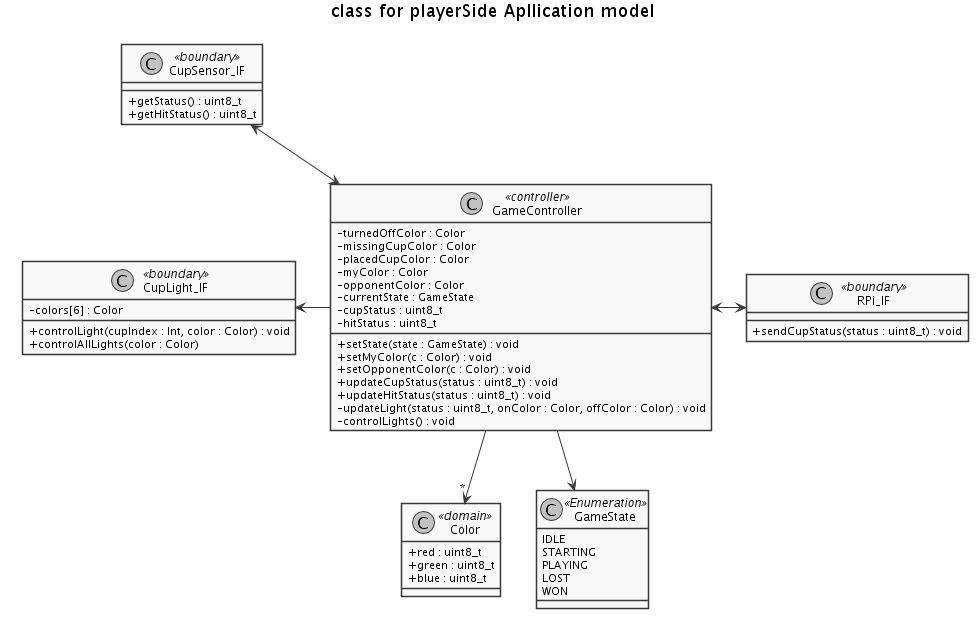
\includegraphics[width=1.2\textwidth]{Arkitektur/Softwarearkitektur/Applikationsmodel/PlayerSide/graphics/classDiagram.png}
    }
    \caption{Klassediagram for playerSideApp}
    \label{fig:CD_PlayerSide}
\end{figure}

Som tidligere beskrevet modtager GameController information fra RPi om hvilken tilstand playerside skal være i. Det er derfor relevant at udvikle en tilstandsmaskien, som ses på figur \ref{fig:playerSide_SM}. Som det ses på diagrammet skifter tilstandsmaskinen tilstand, når der kaldes metoden setState. Denne metode kaldes af RPi\_IF klassen når der modtages en ny tilstand. I tilstandene STARTING og PLAYING, som svarer til UC1 og UC2, skal lyset styres på baggrund af hvilke kopper der er placeret, og i PLAYING hvilke kopper som er ramt. Dette gøre som en del af Controller metoden som tjekker attributterne cupStatus og hitStatus. Lyset styres vha. controlLight funktionen i CupLight\_IF klassen. Disse attributer opdateres ved at CupSensor\_IF klassen kalder updateCupStatus og updateHitStatus. Dette kan ses som en del af sekvensdiagrammerne for UC1 og UC2. I tilstandene IDLE, WON og LOST skal lyset kun styres ved entry af tilstandene. Dette gøres vha. controlAllLights funktionen i CupLight\_IF klassen.      

\begin{figure}[H]
    \centering
    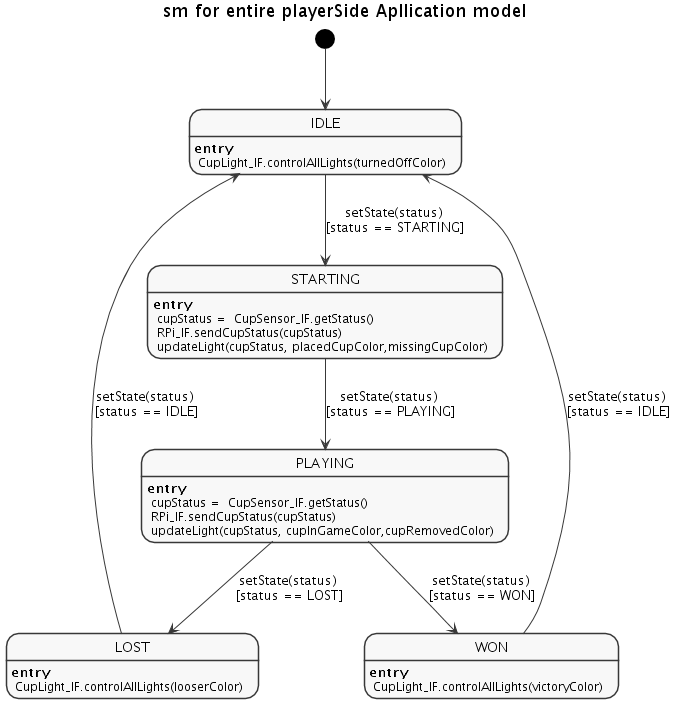
\includegraphics[width=0.9\textwidth]{Arkitektur/Softwarearkitektur/Applikationsmodel/PlayerSide/graphics/state.png}
    \caption{Tilstandmaskine for playerSideApp}
    \label{fig:playerSide_SM}
\end{figure}


\subsubsection{RPiApp}
I det følgende afsnit beskrives softwarearkitekturen for RPiApp. Den fulde dokumentation for arkiteturen kan ses i bilaget \textbf{Arkitektur} \fullref{arch:sec:rpiapp_application_model} \\
Softwareapplikationen består af forskellige sprog, men generelt er objektorienteret C++ benyttet. I forlængelse af dette, er der lavet en applikationsmdel til at beskrive strukturen og forløbet for applikationens objekt-orienteret softwaresystem. I de næste afsnit ses klasse-, sevkens og tilstandsdiagrammer for use case 1-4. \\\\
\textbf{Klassediagram for UC1 til UC4}\\
Traditionelt ville man udarbejde et klassediagram for hvert use case for systemet, men gennemstrømningen for systemet (Use cases) er en forlængelse af hinanden, overvejende use case 1 til 3. Figur \ref{fig:CD_RPI_RAP} viser klassediagrammet for UC1 til UC4
\begin{figure}[H]
    \centering
    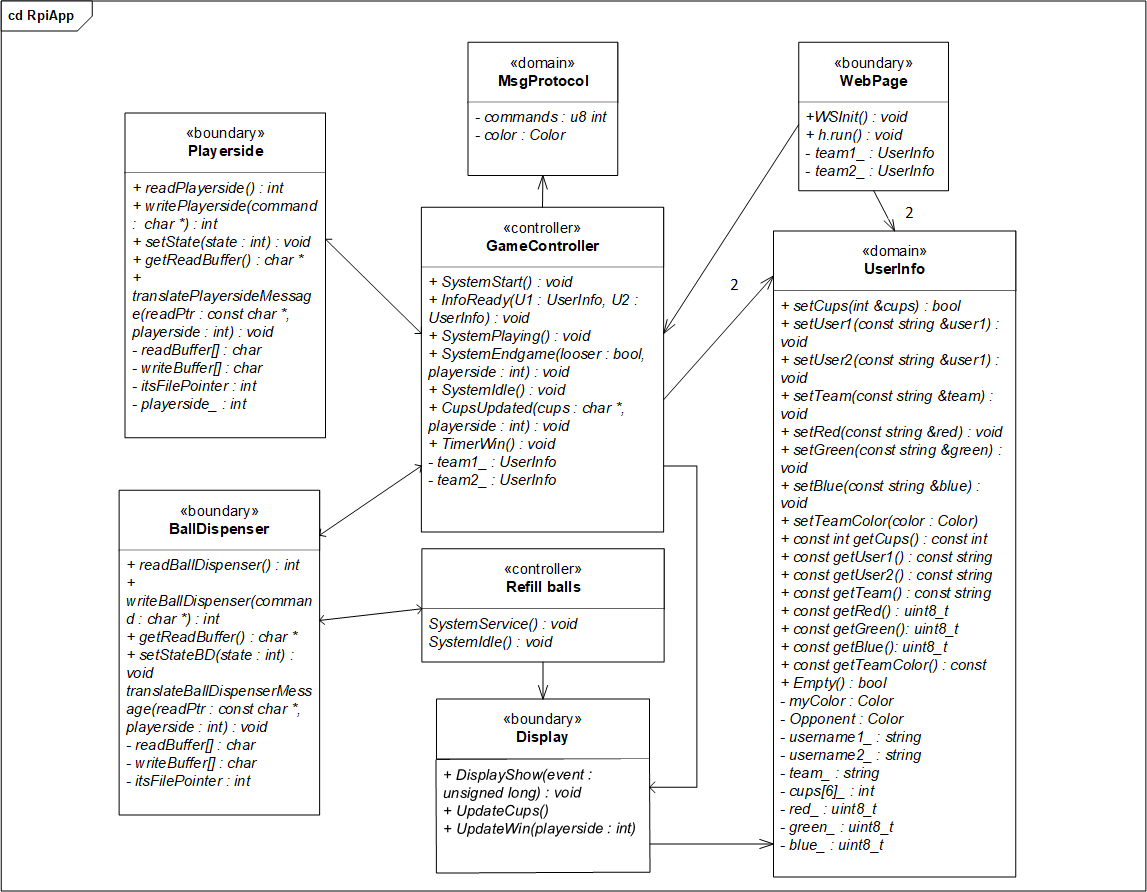
\includegraphics[width=\textwidth]{Arkitektur/Softwarearkitektur/Applikationsmodel/RPi/graphics_RPi/Class.png}
    \caption{Klassediagram for RPi}
    \label{fig:CD_RPI_RAP}
\end{figure}
\textbf{Controller:  GameController}\\
GameController er den centrale controller klasse for use case 1 - 3. Den sørger for at sende og modtage data gennem boundary klasserne Playerside og BallDispenser. Alt modtaget data bliver evalueret i GameController og sendt videre i overensstemmelse med protokollen og use case flow. Klassen varetager alt logikken og de flest beslutninger i systemet.\\\\
\textbf{Boundary:  PlayerSide}\\
Grænseflade til udveksling af data mellem RPi og Playerside-enhed. Klassen bruger filoperationer til at interagere med Kernal Space driveren - her søges for at omsætte en kommando modtaget fra en Playerside-enhed til MsgProtocol kommando, som kan behandles af GameController og vice versa.\\\\
\textbf{Boundary:  BallDispenser}\\
Grænseflade til udveksling af data mellem RPi og BallDispenser-enhed. Klassen bruger filoperationer til at interagere med Kernal Space driveren - her søges for at omsætte en kommando modtaget fra en BallDispenser-enhed til MsgProtocol kommando, som kan behandles af GameController og vice versa.\\\\
\textbf{Boundary: WebPage}\\
Klassen udgør serversiden af hjemmesiden. Den gør brug af et WebSocket API og står for at håndtere beskeder, som modtages fra client. Den skal initialisere to objektere af UserInfo klassen og sende dem til GameController klassen.\\\\
\textbf{Domain: UserInfo}\\
Klassen indeholder informationer, som repræsenterer Playersides (De fysiske spillersider). Klassen skal således indeholde alle informationer, som er relevante for et givet hold.\\\\
\textbf{Boundary: Display}\\
Boundary klassen Display repræsenterer den grafiske brugeroverflade. Den har til opgave at styre det fysiske display, som er koblet til RPi. \\\\
\textbf{Sekvensdiagram for UC1}\\
GameControlleren er logikken i systemet og tager alle de store beslutninger. Dens hovedfunktioner er at modtage data fra de enkelte delsystemer, som BallDispenser og Playerside, og agerer i forhold til dette. Boundary klasserne Playerside og BallDispenser læser konstant efter nyt data - når read-operationen kaldes, 'sover' processen indtil data er modtaget. Når nyt data er modtaget, behandles det og videresendes til GameController. \\\\
I forhold til spillets gang sender GameController information til delsystemerne via boundary klasserne. Fx sender den stadier til Playerside (IDLE) og BallDispenser (DISPENSE\_OFF). Den bruger to UserInfo objekter til at symboliserer to spillende hold, og kontrollere gennem dem, hvornår spillet er ovre (og andre informationer). \\\\
\begin{figure}[H]
    \centering
    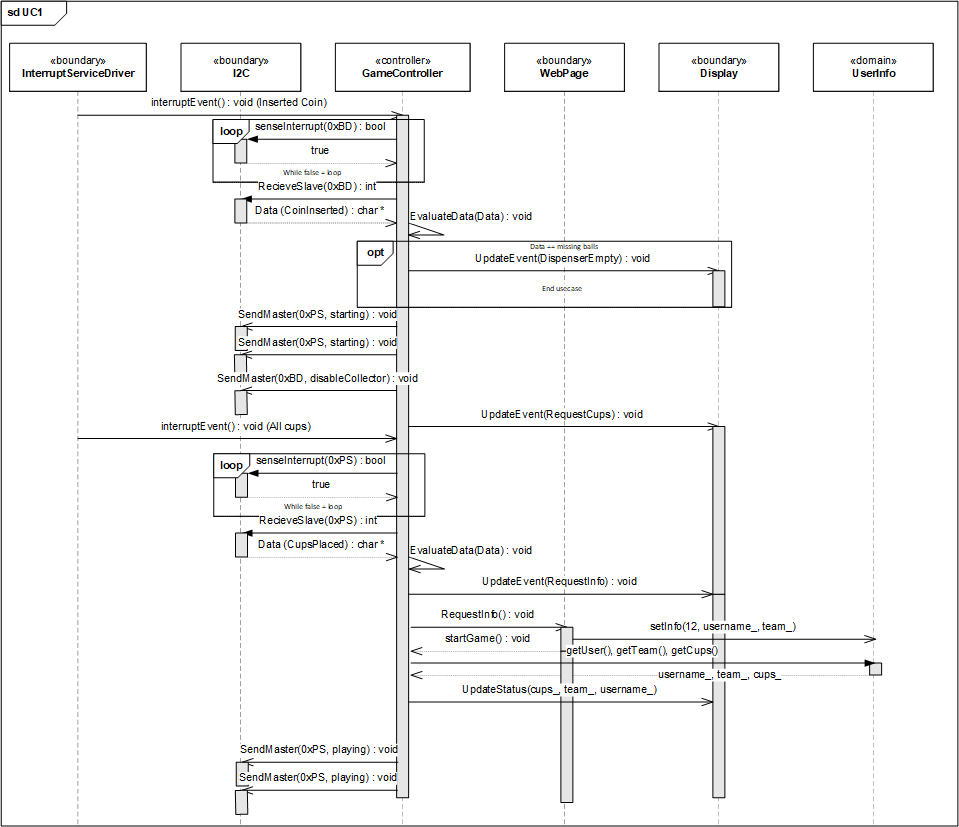
\includegraphics[width=\textwidth]{Arkitektur/Softwarearkitektur/Applikationsmodel/RPi/graphics_RPi/UC1_SD.png}
    \caption{Sekvensdiagram for UC1. Hver opmærksom på at mellemrummet mellem eksekverings specifikation 'boksen' indikerer en pause i processen; fx processeson 'sover', når der læses fra "BallDispenser" eller der ventes information fra WebPage}
    \label{fig:UC1_SD_RPi_RAP}
\end{figure}
Det kan ses på sekvensdiagrammet for UC1, at når funktionen readBallDispenser() eller readPlayerside() kaldes, så sover processen. Read og write operationerne i User Space er tilknyttet en Kernal Space driver. Device driveren er linket mellem det integrede hardware i Rasberry Pi W Zero og User Space applikationen - driveren beskrives kort i det næste afsnit. 

\subsubsection{i2c\_interruptDriver}
I2c\_interruptDriver er den driver, som bruges på RPI'en. Den sørger for at sende beskeder og læse fra de forskellige PSoC's i systemet. På figur \ref{fig:driver_sekvensdiagram} ses et sekvens diagram, der beskriver det samspil, der er mellem userspace, kernelspace samt PSoC enhederne i systemet. 
\begin{figure}[H]
    \centering
    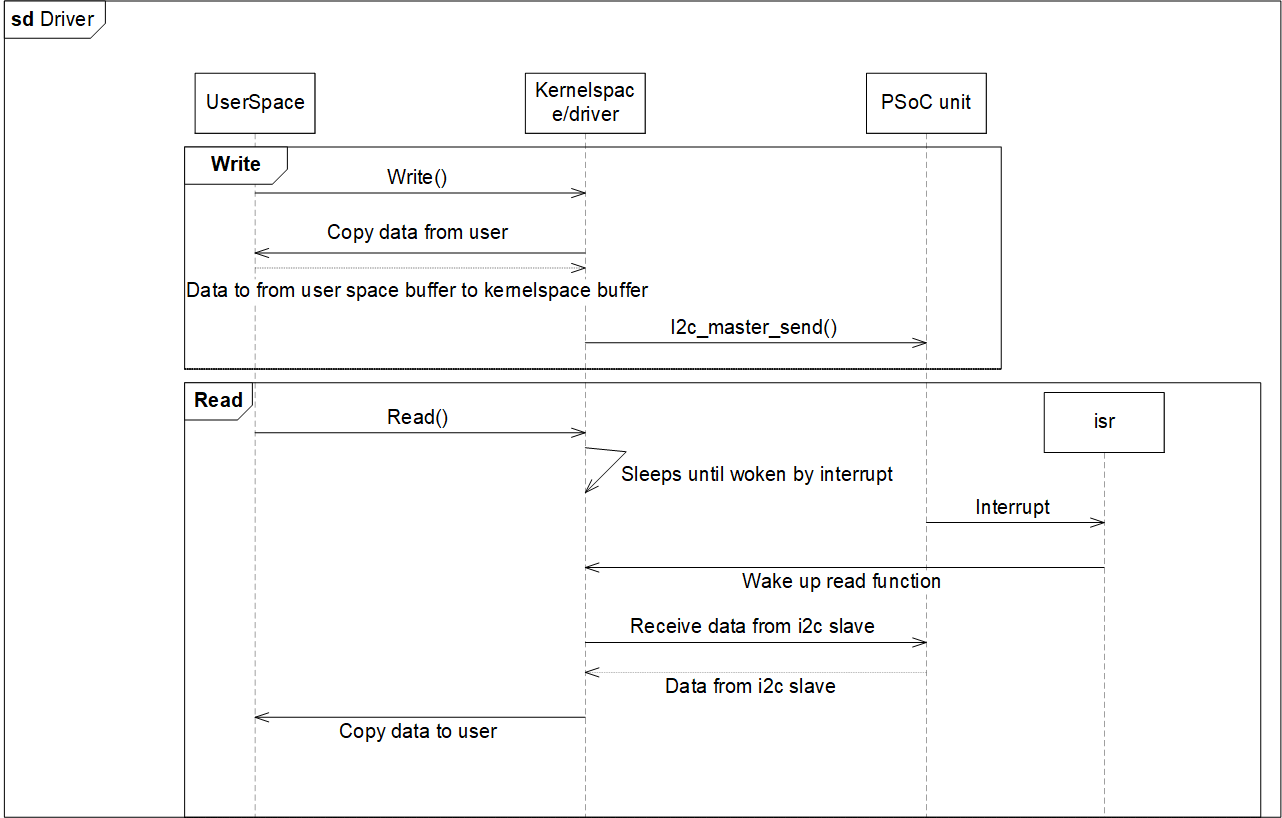
\includegraphics[width=\textwidth]{Rapport/Arkitektur/graphics/driver_sekvensdiagram.png}
    \caption{Her ses sekvensdiagram for driver, hvor samspillet mellem userspace, kernelspace og PSoC's(i2c slaver) vises.}
    \label{fig:driver_sekvensdiagram}
\end{figure}





\subsubsection{BallDispenserApp}
I dette avsnittet presenteres software arkitekturen for BallDispenser, for den fulle dokumentasonen refereres der til \textbf{Systemarkitektur} \fullref{arch:sec:balldispenser_application_model}. Applikasjonen er skrevet i C for å kunne kjøres på en PSoC. Under vil klasse, sekvens og tilstands diagrammene til UC1 og UC4 bli presentert.\\\\
\textbf{Klasse diagram BallDispenserApp}\\
\begin{figure}[H]
    \centering
    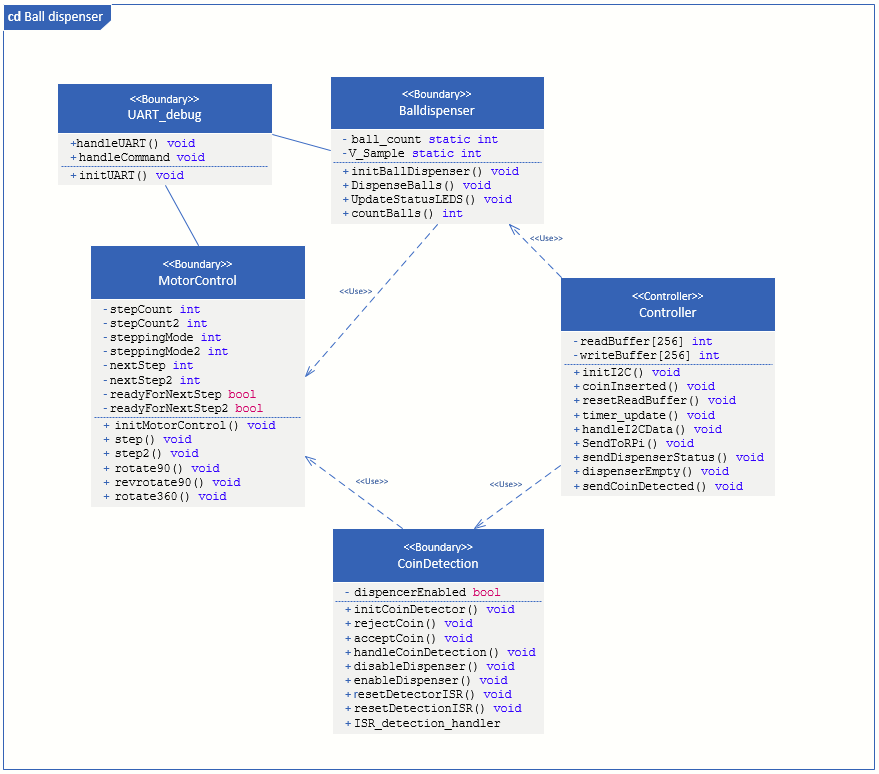
\includegraphics[width=\textwidth]{Rapport/Arkitektur/graphics/CDBolddispenser.png}
    \caption{Klassediagram for BallDispenser}
    \label{fig:BallDipKlasse}
\end{figure}

\textbf{Balldispenser - State machine}\\
\begin{figure}[H]
    \centering
    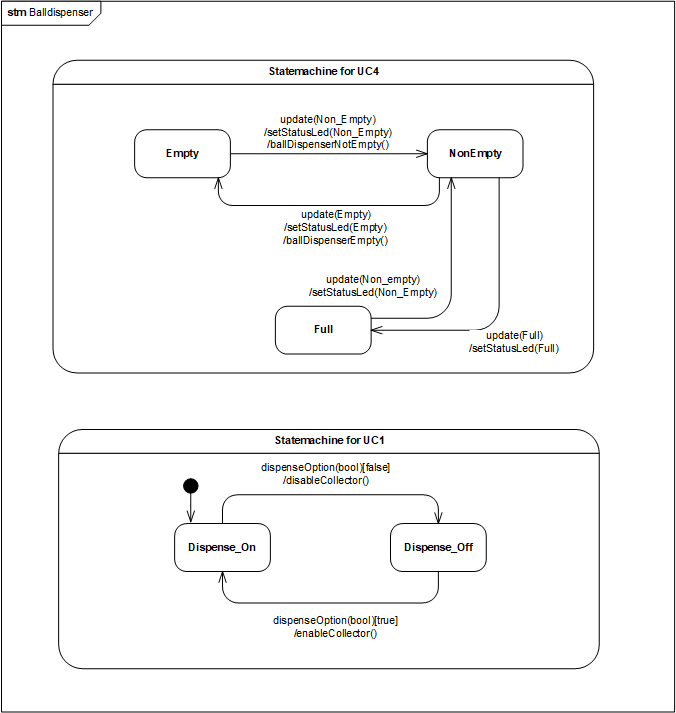
\includegraphics[width=\textwidth]{Arkitektur/Softwarearkitektur/Applikationsmodel/BallDispenser/graphicsBallDispenser/ApplikationsmodelBolddispenserstm.PNG}
    \caption{BallDispenser State machine}
    \label{fig:my_label}
\end{figure}
Denne figuren viser stadiene for BallDispenser. Den består av to mindre state machines, en som styrer balldispenser og en som styrer CoinDispenser. CoinDispenser enable/disable styres av RPi via I2C. BallDispenser STMen styres av countBalls funksjonen. Dette dokumenteres grundigere i \textbf{Systemarkitektur} \fullref{arch:sec:BallDispSTM}.

\textbf{Sekvensdiagram for UC1}\\
\begin{figure}[H]
    \centering
    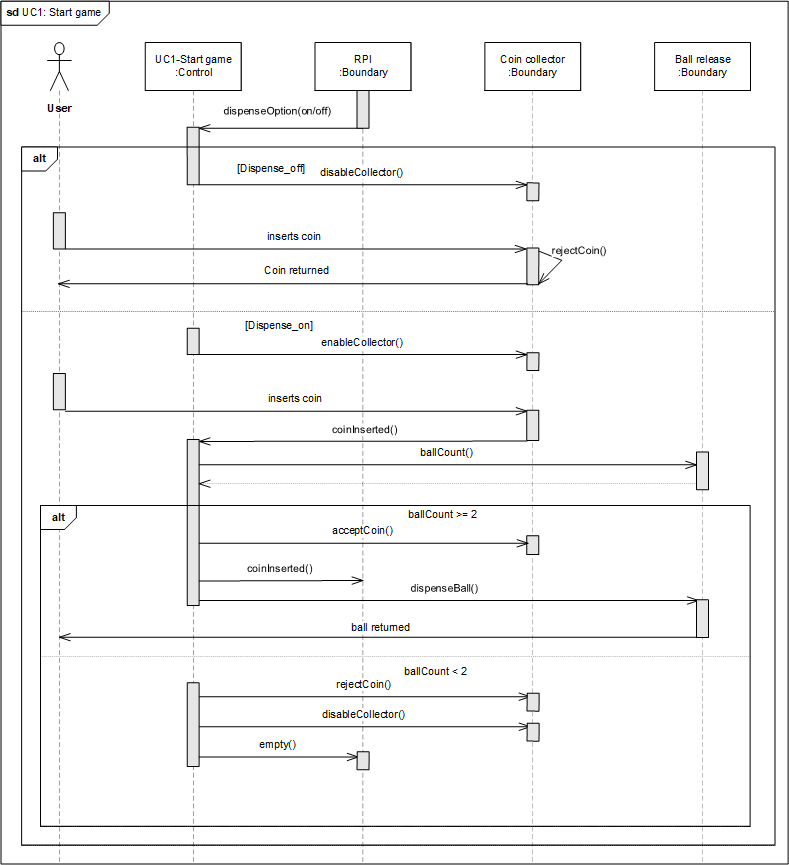
\includegraphics[width=\textwidth]{Arkitektur/Softwarearkitektur/Applikationsmodel/BallDispenser/graphicsBallDispenser/sdUC1.png}
    \caption{Sekvensdiagram for UC1 (Balldispenser)}
    \label{fig:BallDispScUC1}
\end{figure}

Ut fra sekvensdiagrammet (figur \ref{fig:BallDispScUC1}) kan det sees hvis en bruker innsetter en mynt i systemet mens det er i staten dispense\_off så kalder den rejectCoin() og fortsetter å vente. Mens hvis den er i dispense\_on skjekker den hvor mange baller som er igjen, hvis det det er nåkk akseperer den mynten, sender en beskjed til RPi og dispenserer baller. Hvis det ikke er nåkk avviser den mynten, disabler CoinCollector og sender beskjed til RPI.\\\\

\textbf{Sekvensdiagram for UC4}\\
\begin{figure}[H]
    \centering
    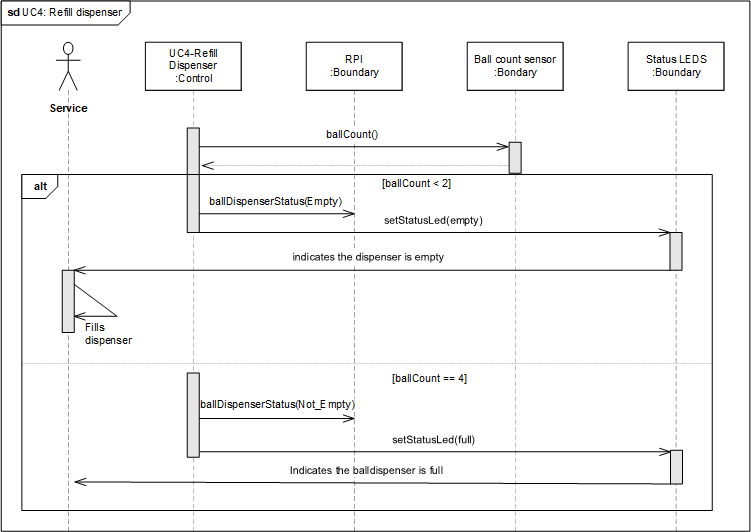
\includegraphics[width=\textwidth]{Arkitektur/Softwarearkitektur/Applikationsmodel/BallDispenser/graphicsBallDispenser/sdUC4.png}
    \caption{Sekvensdiagram for UC4 (Balldispenser)}
    \label{fig:BallDispScUC4}
\end{figure}

Ut fra sekvensdiagrammet (figur \ref{fig:BallDispScUC4}) kan det sees den starter med ballCount(), hvis den returnerer en verdi som er lavere enn 2 sender den beskjed til Rpien om at den er tom og indiker det til service medarbedidern ved å endre på status LEDene. Etter dispenseren har blitt fylt kalles ballCount() igjen og LEDene endres slik de viser dispenseren er full.

\end{document}